%!TeX root=../tese.tex
%("dica" para o editor de texto: este arquivo é parte de um documento maior)
% para saber mais: https://tex.stackexchange.com/q/78101

% Vamos definir alguns comandos auxiliares para facilitar.

% "textbackslash" é muito comprido.
\newcommand{\sla}{\textbackslash}

% Vamos escrever comandos (como "make" ou "itemize") com formatação especial.
\newcommand{\cmd}[1]{\textsf{#1}}

% Idem para packages; aqui estamos usando a mesma formatação de \cmd,
% mas poderíamos escolher outra.
\newcommand{\pkg}[1]{\textsf{#1}}

% A maioria dos comandos LaTeX começa com "\"; vamos criar um
% comando que já coloca essa barra e formata com "\cmd".
\newcommand{\ltxcmd}[1]{\cmd{\sla{}#1}}

\chapter{Arquitetura}
\label{chap:arquitetura}

\enlargethispage{-.5\baselineskip}

\section{Arquitetura Antiga}

A arquitetura estava dividida em três partes: o banco de dados PostgreSQL, o back-end em Django e o front-end em React, todas agrupadas em um mesmo repositório. Cada instituto possuía seu código exclusivo e uma instância dedicada para o banco de dados. Além disso, eram criados containers Docker para cada camada da arquitetura, resultando em três containers distintos: um para o front-end, outro para o back-end e o último para o banco de dados. Esses containers eram então instanciados no serviço de nuvem da AWS chamado EC2, que cria máquinas virtuais para a aplicação. Assim, uma única VM (máquina virtual) era responsável por conter o back-end, front-end e banco de dados de um instituto específico. Do ponto de vista técnico, o sistema anterior era estruturado em uma arquitetura monolítica, onde o front-end e o back-end estavam intimamente vinculados em um único código fonte.

A figura a seguir exibe, de forma geral, a estrutura do sistema para um instituto:

\begin{figure}[!htb]
\centering
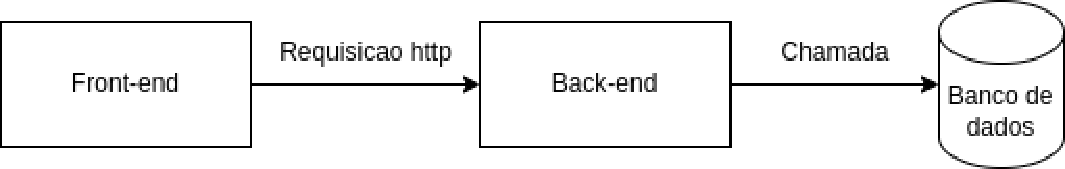
\includegraphics[width=0.75\textwidth]{figuras/arquitetura_antiga.pdf}
\caption{Estrutura geral antiga}
\label{estrutura_antiga}
\end{figure}

Considerando o modelo de arquitetura apresentado na Figura \ref{estrutura_antiga}, o procedimento para inserir um novo instituto exigia a replicação integral do código: front-end, back-end e a criação de um novo banco de dados independente. Isso resultava na criação separada de cada front-end, originando pequenas particularidades no desenvolvimento, embora os códigos fonte seguissem um modelo com considerável replicação entre os institutos. No back-end, a cada novo instituto, era necessário criar uma nova instância com código idêntico aos anteriores. O mesmo padrão era aplicado ao banco de dados, ou seja, uma nova instância era criada para cada instituto adicional.

Essa estrutura de código replicado ocasionou vários problemas. A manutenção do projeto tornou-se progressivamente mais complexa, trabalhosa e propensa a erros, uma vez que cada alteração demandava modificações em cada instância de código individualmente. Por exemplo, ao inserir um novo botão em todos os sites, era necessário modificar cada código fonte separadamente, resultando em desafios significativos na manutenção dos sites.

Com a arquitetura anterior, foram desenvolvidos sites para três institutos distintos: FAU, IME e FEARP, o que demandou o uso de três instâncias de máquinas virtuais na AWS. Essa abordagem resultou em um aumento de custos, uma vez que era necessário criar uma nova máquina virtual toda vez que um novo instituto era inserido no projeto. Embora, de acordo com a lógica de escalabilidade horizontal, isso fosse considerado uma qualidade do projeto, percebeu-se que a demanda pelo back-end era relativamente pequena. Portanto, concluiu-se que não seria necessário alocar uma máquina virtual exclusiva para a execução do back-end. A disposição das máquinas virtuais na AWS pode ser visualizada na figura a seguir.

\begin{figure}
    \centering
    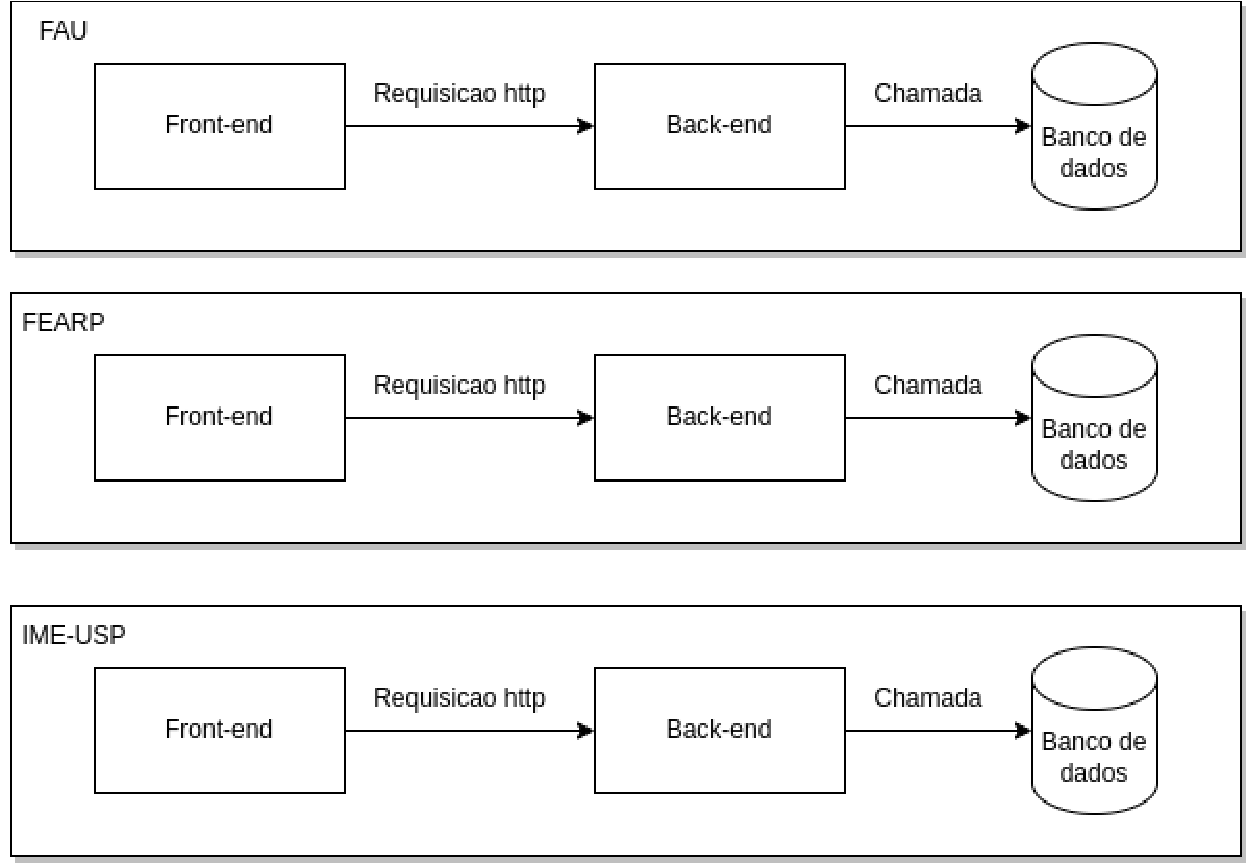
\includegraphics[width=0.75\linewidth]{figuras/arqtuitera_antiga_institutos.pdf}
    \caption{Estrutura antiga com os institutos que foram criados}
    \label{fig:arquitetura-antiga}
\end{figure}

Outra problemática presente na abordagem da arquitetura monolítica é a questão da segurança. A manutenção de todos os componentes agrupados em um único código base implica o compartilhamento do mesmo contexto de segurança. Em outras palavras, isso resulta em uma superfície de ataque maior, uma vez que uma vulnerabilidade em uma parte do sistema pode comprometer toda a plataforma.

Em resumo, a própria arquitetura se tornava um obstáculo para a escalabilidade do projeto, além de apresentar todas as dificuldades burocráticas relacionadas à obtenção de dados. Os custos associados à inclusão de novas unidades envolviam despesas financeiras (AWS), trabalho desnecessário por parte dos desenvolvedores e tempo a ser dedicado.


\section{Arquitetura Atual}

Visando corrigir esses problemas, buscou-se criar uma nova arquitetura que desacoplasse as diferentes partes do projeto. Inicialmente, separou-se o back-end e o front-end em diferentes repositórios para aprimorar a organização do projeto. A arquitetura Headless, que divide as responsabilidades entre o front-end, responsável pela interface de usuário, e o back-end, responsável pelo CMS e pela lógica de negócios, foi identificada como o sistema mais benéfico ao analisar os objetivos do projeto.

Anteriormente, cada instituto possuía um banco de dados próprio gerado dentro de um container Docker. Agora, esses bancos de dados individuais foram consolidados em uma única estrutura, utilizando uma tecnologia chamada RDS da Amazon, que armazena banco de dados PostgreSQL.

Essa nova estrutura de bancos de dados agregados possibilitou a unificação do back-end, uma vez que as requisições dos sites podiam ser filtradas, permitindo direcionar o back-end para o banco de dados apropriado em função dos diferentes tipos de consultas.

Os diferentes back-ends e bancos de dados criados para cada instituto foram unificados. Isso significa que os sites dos institutos poderiam requisitar dados de uma única API, resultando em apenas uma VM na AWS executando o back-end. Essa mudança não apenas reduziu os custos, mas também simplificou o processo de manutenção.

Uma nova camada para o CMS foi criada utilizando o Strapi, sendo responsável por gerir os estilos e estados dos diferentes sites. Nela, era possível armazenar os designs de cada site e modificá-los em tempo de execução. Em outras palavras, possibilitou a unificação do código-fonte do front-end, tornando viável a criação de páginas distintas utilizando a mesma estrutura. Essa nova arquitetura proporcionou facilidade na inserção de novos institutos, além de contribuir para a manutenção dos já existentes.

A figura a seguir (Figura \ref{fig:arquitetura-nova}) representa essa nova estrutura com os antigos institutos.

\begin{figure}
    \centering
    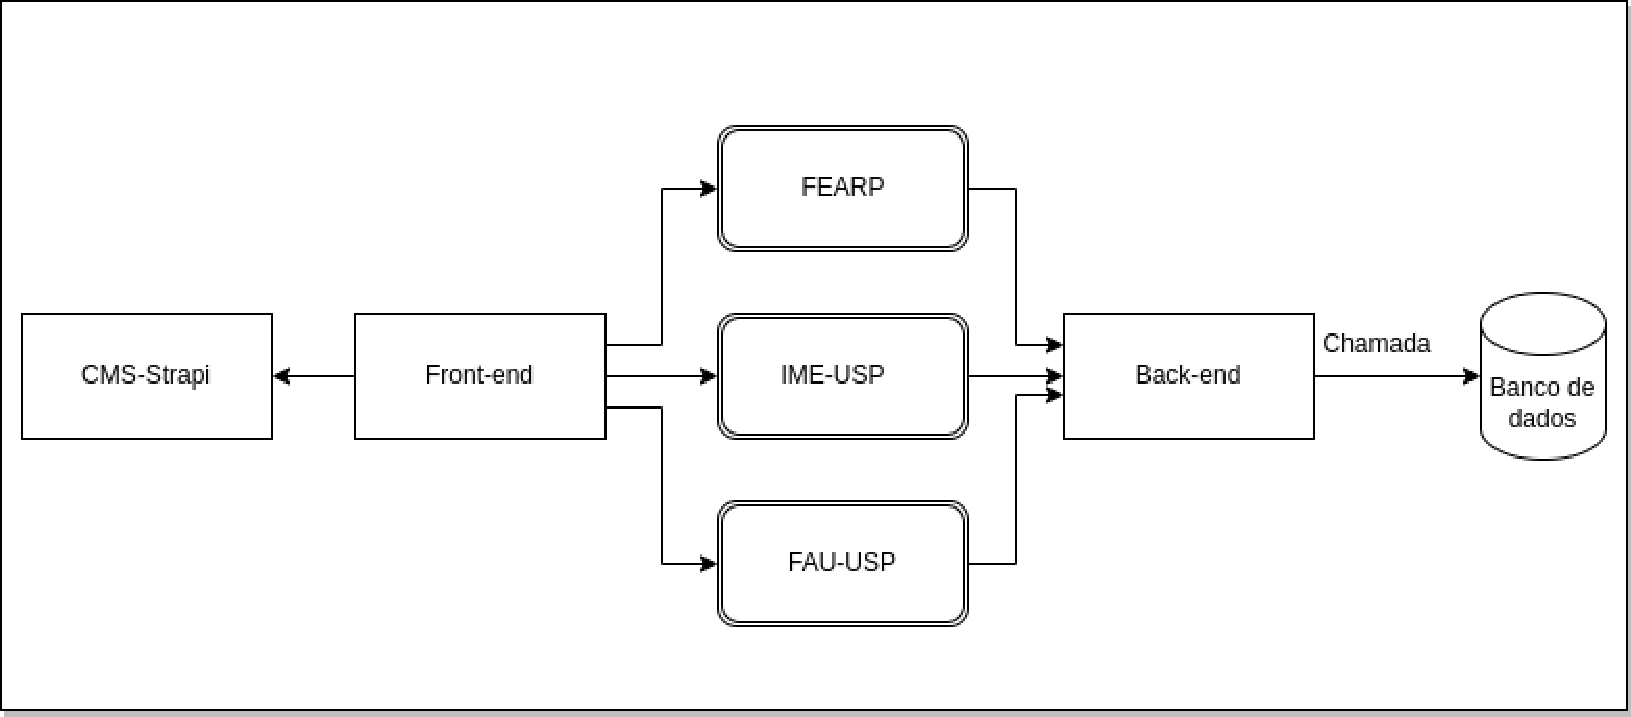
\includegraphics[width=0.75\linewidth]{figuras/nova_arquitetura.drawio-_1_.pdf}
    \caption{Estrutura novas com os institutos que foram criados}
    \label{fig:arquitetura-nova}
\end{figure}

Pela análise das imagens \ref{fig:arquitetura-antiga} e \ref{fig:arquitetura-nova}, é possível compreender melhor a questão da unificação. Na nova abordagem, há um front-end que realiza uma requisição para o CMS, gerando diferentes designs para os institutos. Quando o site é gerado, ocorre uma requisição para o back-end obter os dados referentes ao instituto em questão, direcionando a API para o banco de dados apropriado.

Atualmente, a instância do front-end utiliza o serviço da Amazon S3, que armazena arquivos e hospeda sites estáticos, como é o caso deste projeto que utiliza ReactJS. Para a hospedagem, basta utilizar a funcionalidade de build do framework, que gera um código HTML e, em seguida, é enviado para o serviço de armazenamento da Amazon. Dessa forma, não é mais necessário utilizar um container e uma VM para executar o front-end.

Portanto, na arquitetura atual, ocorre a build do código, que é o mesmo para todos os institutos, sendo a única diferença a especificação na variável ambiente indicando qual instituto está passando pelo processo.

\section{Opções e escolhas}
    \subsection{Headless CMS}
Um Headless CMS separa o conteúdo da apresentação, fornecendo esse conteúdo por meio de APIs para que os desenvolvedores possam escolher a forma de apresentação. Conceitualmente, o termo "headless" refere-se à separação da cabeça (front-end) do corpo (back-end), de forma semelhante ao Decoupled CMS. Embora ambos apresentem vantagens em aplicações complexas, o headless CMS se destaca ao enviar o conteúdo via API para diversos dispositivos, como dispositivos móveis e Internet das Coisas (IoT).

Ao comparar ambas as abordagens, decoupled e headless, a principal distinção está na flexibilidade de personalização. No atual projeto, em que a principal preocupação diz respeito à possível limitação na personalização, o headless CMS mostrou-se como a melhor alternativa.

Enquanto o decoupled CMS permite a desacoplagem do back-end e front-end, ainda mantendo opções de visualização pré-construídas, o headless CMS garante liberdade para criar interfaces de usuário (front-end) personalizadas para diferentes plataformas. Em outras palavras, a abordagem escolhida oferece total controle sobre a Interface de Usuário (UI), permitindo sua criação a partir do zero. Por outro lado, a outra alternativa proporciona maior flexibilidade em relação ao CMS tradicional, mas apresenta algumas opções pré-construídas.

Em contrapartida, existem algumas desvantagens na abordagem Headless. A escolha por maior flexibilidade de personalização implica maior dificuldade no uso, implementação, manutenção e gerenciamento. No entanto, a equipe responsável pela incorporação do Headless CMS realizou o estudo adequado e superou a curva de aprendizado apresentada.

    %%%%% grafico da curva

    \begin{figure}
        \centering
        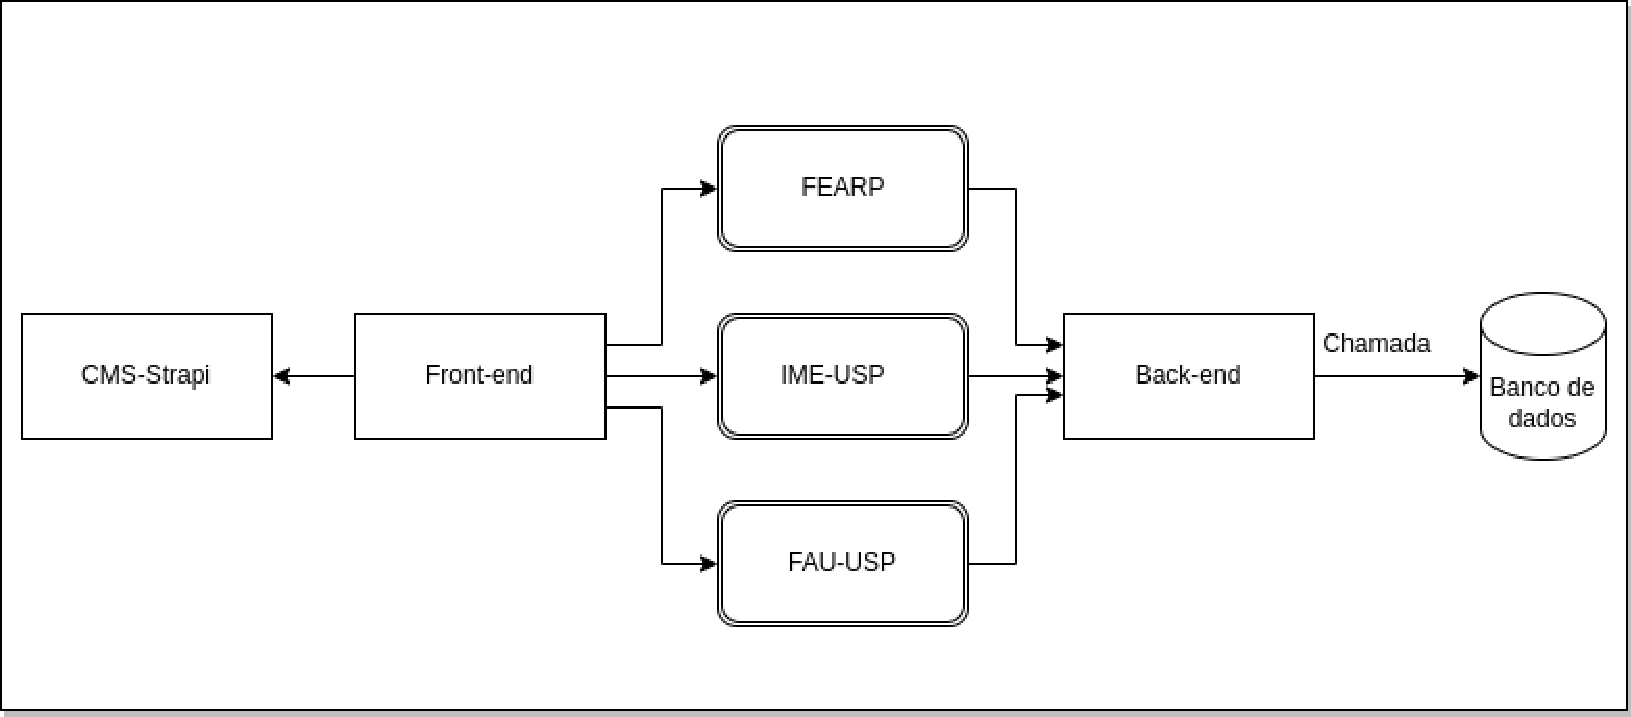
\includegraphics[width=0.75\linewidth]{figuras/nova_arquitetura.drawio-_1_.pdf}
        \caption{Gráfico de aprendizado para cada membro da equipe}
        \label{fig:learning-curve}
    \end{figure}

No gráfico \ref{fig:learning-curve}, foi retratada a porcentagem de domínio da nova tecnologia para cada membro da equipe de desenvolvedores. Observa-se que os membros que possuíam maior conhecimento em relação à linguagem do código herdado apresentaram maior facilidade para se adaptar à nova abordagem. Entretanto, membros cuja linguagem não era familiar no início do desenvolvimento enfrentaram maiores desafios ao lidar com a nova implementação.

Os dados para o gráfico foram coletados no período de 1 de agosto até o início de novembro, com intervalos aproximados de duas semanas entre cada coleta.

Outro fator determinante na escolha da abordagem Headless CMS foi a situação atual das empresas no mercado de trabalho. No início do projeto, foi realizada uma reunião com desenvolvedores de plataformas web de algumas empresas, onde o Strapi foi indicado como a melhor ferramenta para incorporar o sistema headless no projeto.

    Em conclusão, a adoção de um Headless CMS, que separa o conteúdo da apresentação, revelou-se uma escolha estratégica para o atual projeto. Conceitualmente, a abordagem "headless" transcende a metáfora de separar a cabeça (front-end) do corpo (back-end), oferecendo uma vantagem crucial ao enviar o conteúdo através de APIs para diversos dispositivos, como dispositivos móveis e Internet das Coisas (IoT). A comparação entre as abordagens decoupled e headless destacou a principal distinção na flexibilidade de personalização, sendo que o Headless CMS proporcionou a liberdade desejada para criar interfaces de usuário personalizadas para diferentes plataformas. Embora esta escolha tenha apresentado desafios em termos de dificuldade de uso, implementação, manutenção e gerenciamento, a equipe dedicada superou eficazmente a curva de aprendizado, conforme evidenciado no gráfico de aprendizado apresentado. A análise do domínio tecnológico revelou que membros da equipe com conhecimento prévio na linguagem de código herdado tiveram uma transição mais suave para a nova abordagem. Além disso, a consulta inicial a especialistas do mercado de trabalho, que recomendaram o Strapi como a melhor ferramenta para incorporar um sistema headless, solidificou a decisão estratégica. Assim, a escolha do Headless CMS foi respaldada por sua capacidade única de oferecer personalização sem restrições, essencial para atender às demandas específicas do projeto em questão.

    \subsection{Tecnologia Strapi}

   Em relação à escolha tecnológica, as principais alternativas consideradas além do Strapi incluíram o Contentful, o GraphCMS e o Sanity, plataformas de CMS headless amplamente reconhecidas. A decisão de optar pelo Strapi foi fundamentada na aderência à filosofia do Software Livre, destacando-se como um diferencial a sua natureza de código aberto. Este atributo se traduz em uma vantagem significativa, especialmente no que se refere ao extenso ecossistema de plugins. A abertura do código amplia o conjunto de desenvolvedores capacitados a criar plugins, resultando em uma maior diversidade e quantidade de extensões disponíveis.

    É válido mencionar que, embora a escolha pelo Strapi tenha apresentado inúmeras vantagens, algumas desvantagens foram identificadas, embora consideradas menos impactantes pela equipe. Por exemplo, plataformas como o GraphCMS e o Sanity oferecem recursos que aprimoram a colaboração em equipe, como controle de versão e atribuição de tarefas diretamente na plataforma. No entanto, ao explorar o catálogo de plugins do Strapi, foram identificados plugins direcionados ao controle de versão (Content Versioning), enquanto a edição colaborativa poderia ser abordada por meio de um recurso específico, o Strapi Cloud, disponível apenas para usuários pagos.

    Outra consideração abordada refere-se à manipulação de imagens e assets dinâmicos. Embora plataformas como Contentful e Sanity ofereçam abordagens diferenciadas para a manipulação desses dados, no atual contexto do projeto, a presença limitada de imagens, essencialmente relacionadas aos logotipos institucionais, minimizou a relevância desses recursos específicos.

    Em síntese, a escolha do Strapi como plataforma para o desenvolvimento do sistema revelou-se alinhada aos princípios fundamentais do projeto, notadamente no que concerne à adesão à filosofia do Software Livre. A natureza de código aberto do Strapi proporcionou não apenas uma flexibilidade ímpar, mas também um robusto ecossistema de plugins, garantindo uma personalização eficaz e a disponibilidade de uma ampla gama de recursos adicionais. Embora a análise criteriosa tenha evidenciado algumas desvantagens, como a necessidade de recursos pagos para funcionalidades específicas e a abordagem diferenciada de plataformas concorrentes em aspectos colaborativos, esses aspectos foram considerados secundários diante da solidez e adaptabilidade que o Strapi ofereceu ao projeto. A decisão fundamentada na busca pelo equilíbrio entre recursos, filosofia, e necessidades específicas, culminou em uma escolha que não apenas atendeu, mas também enriqueceu os objetivos propostos.